\large{
Di seguito saranno analizzate le possibili tecniche di visualizzazione di grafi ed alberi, come definito anche nel libro "Graph Drawing: Algorithms for the Visualization of Graphs"~\cite{Battista:1998:GDA:551884}  e saranno elencate le modalità di interazione per le rappresentazioni di grafi concludendo infine con una lista di software attualmente in commercio che svolgono tali compiti.
\section{Visualizzazione alberi}
Per quanto concerne la rappresentazione dei grafi ed in particolare degli alberi, ci sono due possibili modelli: node-link e space-filling.
Nella strategia node-link i nodi solo rappresentati come dei punti mentre i link ovvero i collegamenti (gli archi) sono raffigurati come linee. A seconda poi della rappresentazione Node-link scelta si possono avere diverse tipologie di visualizzazione. Ne è un esempio la rappresentazione HV-drawing mostrata nella \textbf{\figurename~\ref{fig:nodeLink}}, in cui gli archi possono essere solamente orizzontali e verticali e che risulta essere molto utile per la rappresentazione di circuiti elettronici.\\
\begin{figure}[!htb]
	\begin{center}
		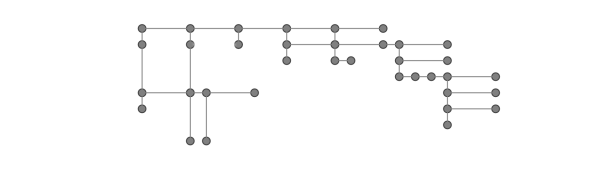
\includegraphics[width=0.8 \linewidth]{figure/nodeLink}
	\end{center}
	\caption{rappresentazione node-link HW drawing di un albero \label{fig:nodeLink}}
\end{figure}
Nella strategia Space-filling si tenta invece di superare i limiti del Node-link che riguardano la gestione non ottimale dello spazio orizzontale in quanto la parte alta della rappresentazione solitamente risulta essere poco densa di informazioni al contrario di quella bassa.\\
Nella strategia Space-filling forme geometriche, solitamente rettangolari, rappresentano i nodi e i figli sono rappresentati da altre forme geometriche inserite all'interno del padre. Questa strategia presenta però vari problemi tra cui la distinzione difficile di tagli orizzontali da quelli verticali e la gestione non ottimale di alberi di grande profondità. Nella \textbf{\figurename~\ref{fig:spaceFilling}} sono mostrate alcune rappresentazioni diverse che seguono la strategia Space-filling.
\begin{figure}[!htb]
	\begin{center}
		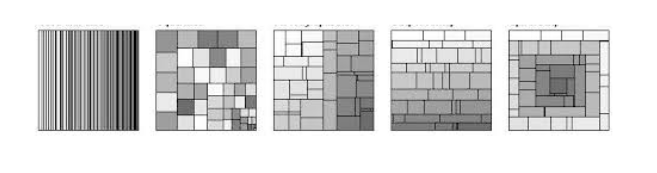
\includegraphics[width=0.9 \linewidth]{figure/spaceFilling}
	\end{center}
	\caption{rappresentazioni Space-filling\label{fig:spaceFilling}}
\end{figure}
\newline
Essendo quest'ultima di difficile lettura solitamente però si opta per la strategia Node-link scegliendo una rappresentazione "layered drawing",di cui ne è un esempio la \figurename~\ref{fig:layered}. In questa rappresentazione i nodi sono organizzati in livelli e per ogni nodo la coordinata y dipende da esso mentre la coordinata x deve esser trovata e dipende: dal numero di figli per ogni livello e dello spazio orizzontale a disposizione per la rappresentazione.
\begin{figure}[!htb]
	\begin{center}
		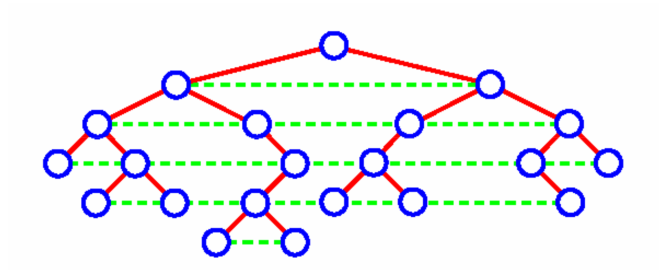
\includegraphics[width=0.9 \linewidth]{figure/layered}
	\end{center}
	\caption{rappresentazione node-Link layered Drawing\label{fig:layered}}
\end{figure}

\section{Visualizzazione grafi}
Il modello principale utilizzato per la visualizzazione di grafi è il \textbf{Force directed} che utilizza una rappresentazione Node-link ed emula il sistema fisico formato da cariche elettriche rappresentate dai nodi e da molle rappresentati dagli archi. L'idea alla base del modello è quella che il raggiungimento di una condizione di equilibro corrisponda ad una rappresentazione grafica gradevole. Ogni rappresentazione di un grafo è dunque formata da due componenti: il \textbf{modello} che descrive le forze in gioco e l'\textbf{algoritmo} ovvero la tecnica che permette di stabilire il punto di equilibrio accettabile. Esistono sono molte varianti del modello Force-directed ma che condividono lo scopo del raggiungimento della condizione di equilibrio. Il primo modello è Barycenter method (Tutte - 1963), seguito dallo Springs \&
electrical forces (Eades - 1984) e dal Magnetic fields (Sugiyama \& Misue - 1995).
\newpage
\begin{figure}[!htb]
	\begin{center}
		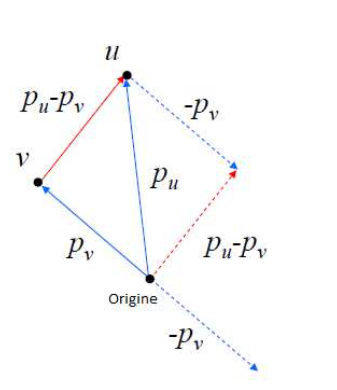
\includegraphics[width=0.4 \linewidth]{figure/baricenter}
	\end{center}
	\caption{Baricenter method\label{fig:baricenter}}
\end{figure}
Il barycenter method è il primo e il più semplice tra i modelli Force directed. Supponiamo di avere due nodi $u$ e $v$ aventi coordinate rispetto ad un punto di origine e consideriamo poi i due vettori $P_u$ e $P_v$ che partono dall'origine ed arrivano a $u$ e $v$. Eseguendo la sottrazione dei vettori $Pu - Pv$, il risultato è il vettore che parte da $v$ e termina in $u$. Questo vettore rappresenta la forza attrattiva di $v$ verso $u$ ed ogni nodo vicino a $v$ attrae $v$ stesso.
$$ F(v)= \sum\limits_{\forall u \in N(v)} (P_u-P_v) $$
La configurazione di equilibrio si ha quando la somma di tutte le forze è pari a 0, $F(v)=0$.\\
Il modello Springs \& electrical forces che permette di avere una rappresentazione simile a quella nella figura \textbf{\figurename~\ref{fig:spring}} Combina forze elettriche e forze meccaniche. Tra i nodi
viene inserita una molla caratterizzata da una certa costante elastica, se avvicino i nodi li respingono, se li allontano la molla li avvicina. La molla tende ad una situazione di equilibrio.
Ad ogni coppia di vertici è possibile associare una molla con lunghezza diversa. In formula:
$$ F(v)= \sum\limits_{(u,v)\in E} f_{uv} + \sum\limits_{(u,v)\in VxV} g_{uv} $$
con g forza repulsiva elettrostatica ed f forza della molla.\\
 \begin{figure}[!htb]
	\begin{center}
		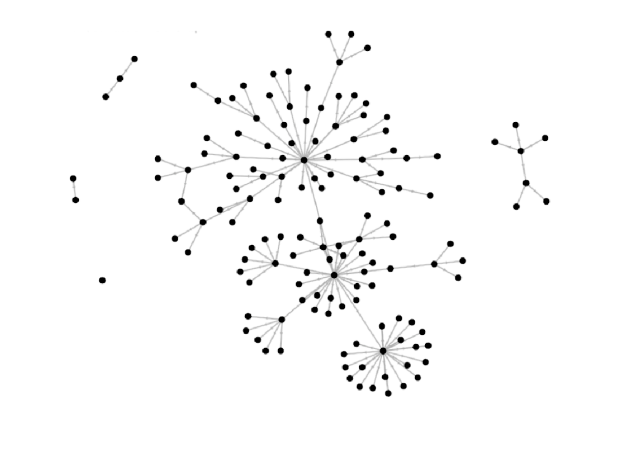
\includegraphics[width=0.8 \linewidth]{figure/spring}
	\end{center}
	\caption{rappresentazione Spring Embedding\label{fig:spring}}
\end{figure}
Il metodo Spring Embedding produce buoni disegni, mette in rilievo anche i cluster di vertici ed enfatizza le simmetrie. Queste proprietà non sono però scientificamente previsti. La sua caratteristica fondamentale è la flessibilità, non ci sono restrizioni sul grafo. A differenza del metodo del baricentro di Tutte qui può essere connesso, non connesso ed è inoltre possibile inserire forze a piacimento.
Per quanto concerne invece la complessità computazionale, il metodo non garantisce il numero di iterazione minimo per poter raggiungere una configurazione di equilibrio ed ogni passo iterativo ha complessità quadratica per i nodi e lineare per tutte le iterazioni avendo quindi un costo complessivo finale $O(n^3)$ senza lasciare però nessuna garanzia sul layout del grafo rappresentato.
Nella rappresentazione Magnetic fields infine le molle vengono magnetizzate in modo che reagiscono
a dei campi magnetici esterni. La molla può essere magnetizzata in modo unidirezionale o bidirezionale.
Per ogni arco, quindi per ogni molla, si va a calcolare la forza 
$$  d(p_u,p_v)^\alpha x sin(\theta)^\beta $$ in cui $\alpha$ e $\beta$ sono due costanti positive e le forze su $u$ e $v$ tendono a stendere la molla lungo il campo magnetico.\\
Le linee di forza del campo magnetico esterno possono essere parallele, radiali e concentriche, potendo quindi dar vita a diverse rappresentazioni grafiche dello stesso grafo.
All'aumentare però del numero di forze in gioco il sistema rallenta e difficilmente il disegno riesce poi a
soddisfarle tutte, la rappresentazione grafica perde in bellezza.

\section{Primitive di interazione per visualizzazioni di grafi}
Per quanto riguarda le interazioni per la rappresentazione dei grafi si elencano qui di sequito quelle elementari:
\begin{itemize}
	\item creazione di un nodo: ogni nodo avrà conoscenza degli archi che sanno collegati ad esso ed avrà delle caratteristiche quali: coordinate nella visualizzazione, colore ed una etichetta che lo contraddistingue; 
	\item creazione di un arco: ogni arco avrà conoscenza dei due nodi che connette;
	\item cancellazione arco: eliminando un arco lo si dovrà rimuovere anche dalla lista degli archi collegati ai nodi che esso connetteva;
	\item cancellazione nodo: ogni qualvolta si elimina un nodo se questo aveva degli archi allora si dovranno cancellare anche i suddetti in quanto un arco è un collegamento tra due nodi.
	\item modifica caratteristiche di un nodo
\end{itemize} 
Definite le interazioni elementari da poter eseguire su un grafo si passa adesso a definire le operazioni più semplici valide per tutte le visualizzazioni non solo di grafi.
Le operazioni semplici che vedremo nel dettaglio sono quelle di select, panning e lo zooming sia spaziale che logico.

Per quando concerne l'operazione di \textbf{select}, mediante una interazione è possibile selezionare un certo numero di punti da rappresentare. Immaginando di avere a disposizione dei dati tabellari riferiti ad un gran numero di nodi ed archi da rappresentare è di grande aiuto poter avere una rappresentazione di un numero di dati selezionato.
\begin{figure}[!htb]
	\begin{center}
		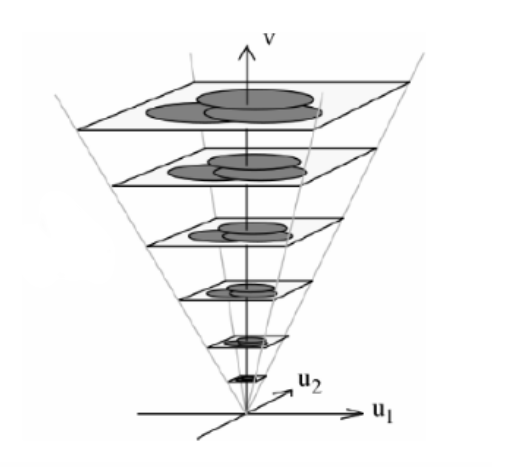
\includegraphics[width=0.7 \linewidth]{figure/zooming}
	\end{center}
	\caption{Operazione di zooming su un piano $<x,y>$\label{fig:zooming}}
\end{figure}
Lo \textbf{zooming} ovvero la possibilità di effettuare un ingrandimento o un ridimensionamento per potersi focalizzare su una parte spaziale di uno oggetto risulta essere una tra le principali primitive di interazione dell'utente. Lo zooming viene utilizzato per per mostrare o nascondere dati, ha significato sia spaziale che logico. E’ possibile eseguire una operazione di zooming e di panning anche contemporaneamente. Immaginiamo di avere un oggetto grafico disegnato su di un piano $<x,y>$ ma replicato su più livelli con grado di ingrandimento diverso lungo v, come mostrato nella \figurename~\ref{fig:zooming}. La distanza dal piano $<x,y>$ determina il grado di zooming mentre il movimento sul piano determina il panning.\\
Tenendo la finestra della visualizzazione bassa riesco a includere dentro ad essa molti oggetti, man mano che si esegue lo zoom out lungo v in un punto anche diverso dal centro, gli oggetti inclusi dalla finestra diminuiscono.
Inoltre un principio da seguire è che per muoversi lungo il piano ad un livello di zoom molto basso, ovvero quando si è lontani dall'origine e si possono vedere pochi oggetti, piuttosto che fare un panning complesso risulta più efficiente eseguire un zoom out avvicinandosi all’origine, un piccolo
panning e poi uno zoom in sino al punto di arrivo sullo stesso piano iniziale come mostrato nella \figurename~\ref{fig:panning}
\begin{figure}[!htb]
	\begin{center}
		\hspace{-1 cm}
		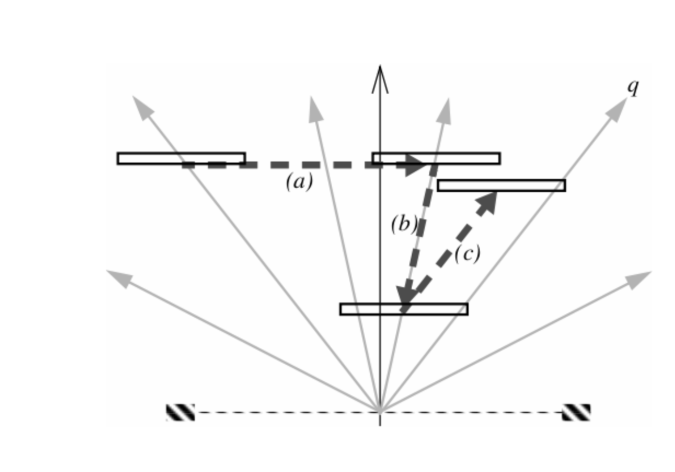
\includegraphics[width=1 \linewidth]{figure/panning}
	\end{center}
	\caption{Operazioni di panning e zooming su un piano $<x,y>$\label{fig:panning}}
\end{figure}

Per terminare con le primitive delle operazioni \textit{semplici} sarebbe necessario nominare anche il labelling ovvero l'operazione che grazie ad una interazione spesso con un tempo di risposta dell'ordine del secondo porta ad una etichettatura di un oggetto del grafo. Anche il labelling però risulta comunque una forma di zooming poiché impiegando una interazione si mostra nella rappresentazione un numero di dati più elevato come fosse uno zooming focalizzato su tutta la visualizzazione.\\
Dalle primitive di integrazione che portano alle operazioni più semplici e pressoché necessarie in ogni visualizzazione saranno ora viste nel dettaglio alcune operazioni, date comunque dall'interazione uomo-macchina con le modalità descritte prima, definibili di completezza per un sistema.
Di grande importanza infatti rappresentano la possibilità da parte dell'utente e della sua interazione di riconfigurare e di eseguire un encode dei dati.
Per quanto concerne la \textbf{riconfigurazione}, questa operazione è definita come la possibilità mediante una interazione di poter cambiare gli attributi o i dati visualizzati.E’ in questo modo possibile modificare cosa visualizzare, cambiando gli intervalli, la scala o ordinare i dati.
L'\textbf{encode }invece è definito come una modifica della visualizzazione e non dei dati. Solitamente mediante una operazione di encode si cambia il tipo di visualizzazione passando, come mostrato a titolo di esempio nella figura \figurename~\ref{fig:pieToBar}, da una rappresentazione a diagramma a barre ad una torta. Include anche operazione di modifica sui colori, sulle forme e l’orientamento della visualizzazione.
\begin{figure}[!htb]
	\begin{center}
		\hspace{-3.5 cm}
		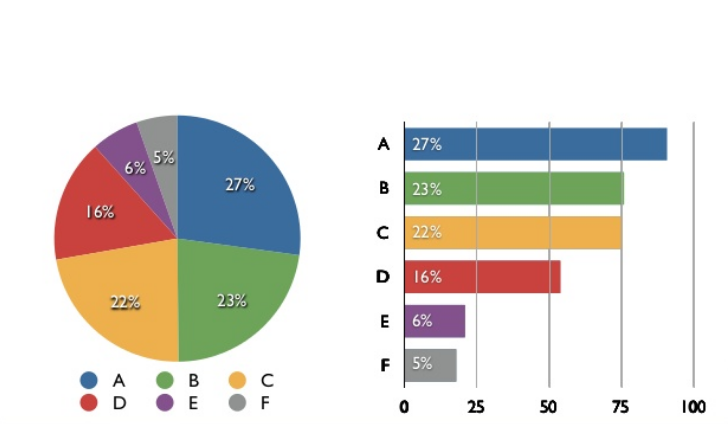
\includegraphics[width=1 \linewidth]{figure/pieToBar}
	\end{center}
	\caption{Esempio di encoding da un diagramma a torta ad uno a barre\label{fig:pieToBar}}
\end{figure}
La primitiva che risulta comunque essere maggiormente complessa da realizzare è però proprio quella su cui si basano le proprietà di creazione e di modifica di un oggetto facente parte del grafo: la \textbf{connessione}.
Riuscire infatti a dare la possibilità di eseguire con una interazione una operazione di connessione non solo a livello grafico mediante la visualizzazione ma anche dei dati risulta essere uno degli obiettivi più complessi da raggiungere.\\
Per concludere la digressione introduttiva delle primitive di iterazione e delle operazioni eseguibili mediante le stesse e per completezza si vuol dare la definizione della primitiva di filtraggio.
Il \textbf{filtraggio} è l’operazione che permette di mostrare un sottoinsieme di dati secondo certe regole, ovvero ciò che può esser definito come uno zoom semantico. Può far uso di query tradizionali ma anche di query dinamiche. Con le query dinamiche l’operazione è rapida, immediata,cambiando un parametro la visualizzazione cambia di conseguenza, ed è immediatamente reversibile, i tempi di attesa sono minori del decimo di secondo. Nelle query classiche invece l’attesa è più alta, l’utente forma le query che vengono eseguite sulla base di un evento, che nel nostro caso risulta essere la pressione di un bottone. Tipicamente però i filtraggi eseguiti con le query dinamiche non sono complesse e le operazioni riguardano tutti i dati. È naturale pero immaginare come aumentando delle dimensioni dei dati l’interazione diviene sempre più lenta.\\ 

\section{Editors per grafi}
Definite le primitive di interazione e le modalità di visualizzazione si passa adesso all'elenco e alla descrizione dei software per la loro creazione.
Attualmente sono disponibili pochi editor \textbf{specifici} per la visualizzazione e anche per la creazione e la conseguente eventuale modifica di grafi. Un esempio famoso ne è Graphviz, software di visualizzazione di grafi open source. Utilizzando Graphviz non si ha però la conoscenza della struttura dati da cui si genera la visualizzazione in quanto rappresenta un mero software grafico.
Altri software per la manipolazione di grafi, ognuno per un particolare interesse nell'ambito della teoria dei grafi, sono:
\begin{itemize}
	\item \textbf{Gephi}: software di visualizzazione ed esplorazione per tutti i tipi di grafi e reti, open source e gratuito.
	\item \textbf{Porgy}: software che mira a progettare rappresentazioni grafiche pertinenti e interazioni adeguate sui grafi dinamici che emergono dai sistemi di riscrittura dei grafi.
	\item \textbf{MS-AGL }:Microsoft Automatic Graph Layout è uno strumento .NET per il layout e la visualizzazione dei grafi open source e basato sullo schema di Kozo Sugiyama(~\cite{108304},~\cite{SUGIYAMA1995217}) .   
\end{itemize}
Esistono poi molti programmi di editor non specializzati e molto più generici come ad esempio Draw.io software di diagrammi online gratuito per la realizzazione di diagrammi di flusso, diagrammi di processo, organigrammi, UML, ER e diagrammi di rete. Anche se non sono presenti molti editor specifici per la creazione di dati relativi ai grafi e la loro conseguente visualizzazione, le primitive di interazione elencate prima sono spesso riscontrabili, anche se in buona parte o con funzioni non totalmente esclusive negli editor non specializzati quali appunto Draw.io.
Un esempio di grafo realizzato mediante uno dei tanti modelli disponibili dal software Draw.io è mostrata nella figura \figurename~\ref{fig:drawIo}
\begin{figure}[!htb]
	\begin{center}
		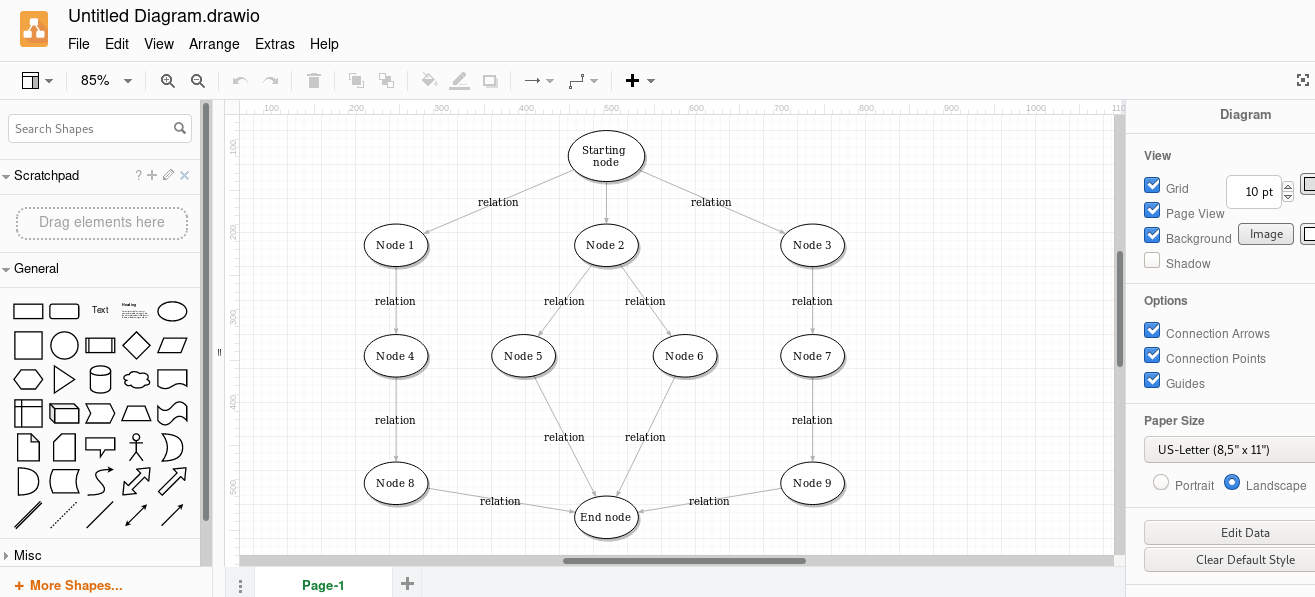
\includegraphics[width=0.8 \linewidth]{figure/drawIo}
	\end{center}
	\caption{interfaccia del software draw.io\label{fig:drawIo}}
\end{figure}
Un altro esempio, sempre non specifico ed esclusivo per la creazione di grafi, è Microsoft Visio,software proprietario per la creazione di grafici e diagrammi, sviluppato da Microsoft per i sistemi operativi Microsoft Windows ed è rilasciato per diverse edizioni di Microsoft Office. Esiste poi la sua controparte \textbf{SmartDraw} utile per la visualizzazione dei dati in grafici ma non supporta molto la creazione di strutture dati come i grafi.
È facile notare come dunque nella teoria dei grafi si abbia la necessità di visualizzare le strutture dati e come questo problema non sia facilmente risolvibile dai software attualmente a disposizione.
}